% !TEX root = cap04_standalone.tex
% Capítulo 4. Área de estudio
% Estructura según índice de la Dra. Lárraga.

\chapter{Área de estudio}
\label{ch:area-estudio}

\begin{resumen}
Este capítulo describe el área de estudio y el conjunto de datos utilizados en la investigación. Se presenta la localización geográfica de la Zona Metropolitana de Querétaro, las características técnicas del conjunto de imágenes (37 años, 1984--2020) obtenidas con \textbf{Google Earth} y su \textbf{herramienta de imagen histórica (línea de tiempo)}, los criterios de calidad y selección aplicados de forma visual al capturar cada año, y el pipeline de preprocesamiento que transforma las imágenes RGB en mapas binarios urbano/no-urbano mediante clasificación LBP+K-Means+SVM.
\end{resumen}

\section{Localización y características del área de estudio}

La Zona Metropolitana de Querétaro se ubica en el centro de México y constituye uno de los polos industriales de mayor crecimiento reciente del país. Su delimitación espacial precisa ---centro del encuadre, extensión cubierta y sistema de referencia--- se detalla en la Tabla~\ref{tab:spatial_criteria}, dentro de la descripción del conjunto de imágenes.

\subsection{Descripción y fuente de datos}

El estudio utiliza una serie anual de \textbf{capturas RGB} (1984--2020, 37 años) sobre la Zona Metropolitana de Querétaro. Las imágenes se obtuvieron con \textbf{Google Earth} en escritorio, usando la \textbf{imagen histórica} (línea de tiempo) para elegir, año a año, una fecha con baja nubosidad visible y buen contraste, manteniendo el mismo encuadre. El fondo cartográfico de Google Earth integra, según época, mosaicos que pueden incluir composiciones basadas en sensores tipo Landsat u otras fuentes; en este trabajo \textbf{no} se empleó Google Earth Engine~\parencite{Gorelick2017} ni descarga masiva por API. La elección de Querétaro se sustenta en su dinámica de crecimiento reciente ---bien documentada para la zona metropolitana~\parencite{Huacuz2018Metropolizacion,DelgadoLopez2018}---, la posibilidad de cubrir 1984--2020 con la misma ventana de visualización y su relevancia como polo industrial en el centro de México, dentro de la expansión urbana que el país arrastra desde los años setenta~\parencite{Montejano2023}.

Tras el preprocesamiento, cada año queda como matriz RGB de \textbf{$1{,}792 \times 3{,}024$} píxeles (del orden de $5{,}4 \times 10^{6}$ píxeles por imagen) en formato PNG; los metadatos de cobertura y tamaño se resumen en la Tabla~\ref{tab:acquisition_stats}.

\section{Adquisición y conformación del conjunto de imágenes}

La adquisición siguió un \textbf{protocolo manual replicable} ---misma ventana geográfica y criterios visuales de calidad en cada año--- orientado a obtener una serie temporal homogénea para estudiar la forma espaciotemporal del crecimiento urbano a partir de percepción remota, en la línea de trabajos que miden esa dinámica desde imágenes~\parencite{Herold2003}. La herramienta fue \textbf{Google Earth} en escritorio, elegida por tres razones prácticas: da acceso a la \textbf{imagen histórica} año con año sobre la misma área, ofrece una interfaz visual inmediata para evaluar nubosidad y nitidez antes de capturar, y hace viable construir la serie sin infraestructura de acceso a API ni \textit{scripts} de descarga. La contrapartida es que la repetibilidad depende de mantener la misma escala, orientación y encuadre entre capturas, y de registrar manualmente la fecha elegida en cada año.

\subsection{Criterios de selección temporal y de calidad}

La serie se diseñó atendiendo a criterios temporales y de calidad de imagen:

\begin{enumerate}
	\item \textbf{Cobertura temporal completa}: 1984--2020 (37 años), suficiente para abarcar varios ciclos de crecimiento urbano.
	\item \textbf{Resolución temporal anual}: una imagen representativa por año, sin años omitidos, para mantener consistencia estacional a lo largo de la serie.
	\item \textbf{Período de adquisición}: imágenes capturadas preferentemente en temporada seca (noviembre--abril), con una meta equivalente a $<10\%$ de cobertura de nubes evaluada por inspección visual.
	\item \textbf{Consistencia geométrica e intensidad}: mismo zoom, orientación y región de interés entre años (con ajuste fino a la cuadrícula en el preprocesamiento) y ausencia de saturación evidente en los canales RGB.
\end{enumerate}

\subsection{Criterios de selección espacial}

\begin{table}[h]
\centering
\caption{Parámetros de selección espacial del conjunto de imágenes.}
\begin{tabularx}{\textwidth}{|>{\raggedright\arraybackslash}p{0.26\textwidth}|X|}
\hline
	\textbf{Parámetro} & \textbf{Especificación} \\
\hline
Área de estudio & Zona Metropolitana de Querétaro. \\
Herramienta y modo & Google Earth en escritorio; adquisición \textbf{manual} con la \textbf{imagen histórica} (línea de tiempo). No se utilizó Google Earth Engine ni descarga masiva por API. \\
Centro del encuadre (aprox., WGS84) & $20{,}59^\circ$\,N, $100{,}39^\circ$\,W (equivalente aproximado a $20^\circ 35' 25''$\,N, $100^\circ 23' 25''$\,W). \\
Extensión cubierta & Del orden de $25 \times 25$~km en el visor, equivalente a unos $625$~km² (referencia operativa para mantener la misma ventana entre años). \\
Sistema de referencia & El visor opera sobre el elipsoide WGS84 (EPSG:4326); la georreferenciación fina de las capturas se homogeneiza en el preprocesamiento. \\
Resolución aparente & Del orden de $8$--$14$~m/píxel ($\sim 115$~m² por píxel; véase el cálculo en el texto). Depende del \textbf{nivel de zoom} elegido y del \textbf{mosaico cartográfico} que Google Earth muestra en cada fecha; se mantuvo el mismo zoom y orientación entre capturas en la medida de lo posible. \\
Bandas & RGB (exportación o captura de pantalla desde Google Earth). \\
\hline
\end{tabularx}
\label{tab:spatial_criteria}
\end{table}

A partir de estos parámetros puede estimarse una resolución espacial efectiva aproximada. La ventana operativa de unos $625$~km² ($\sim 25 \times 25$~km) se exporta a una rejilla de $1{,}792 \times 3{,}024$ píxeles (Tabla~\ref{tab:acquisition_stats}), de modo que cada píxel cubre del orden de $115$~m²: un lado equivalente cercano a $11$~m/píxel como media geométrica, con un rango por eje aproximado de $8$ a $14$~m/píxel, ya que la rejilla no es cuadrada. Conviene leer esta cifra como un orden de magnitud y no como una distancia de muestreo calibrada: la extensión es una referencia de encuadre, el nivel de zoom y el mosaico subyacente varían entre fechas, y Google Earth remuestrea internamente las teselas. La resolución resultante basta para discriminar la mancha urbana a escala metropolitana ---el objetivo de este trabajo---, pero no para distinguir estructuras individuales finas ni para comparaciones submétricas entre años.

\subsection{Resumen cuantitativo del conjunto de imágenes}

\begin{table}[h]
\centering
\caption{Resumen del conjunto de imágenes anuales capturadas.}
\begin{tabularx}{\textwidth}{|>{\raggedright\arraybackslash}X|r|}
\hline
	\textbf{Métrica} & \textbf{Valor} \\
\hline
Imágenes totales & 37. \\
Cobertura temporal & 1984--2020 (una imagen por año). \\
Criterio de nubes & Meta visual de cobertura inferior al $10$\,\%, evaluada al capturar. \\
Dimensiones finales en el \textit{pipeline} & $1{,}792 \times 3{,}024$ píxeles (homogeneizadas en el preprocesamiento). \\
Tamaño total aproximado & Del orden de $200$~MB. \\
\hline
\end{tabularx}
\label{tab:acquisition_stats}
\end{table}

\begin{figure}[h]
\centering
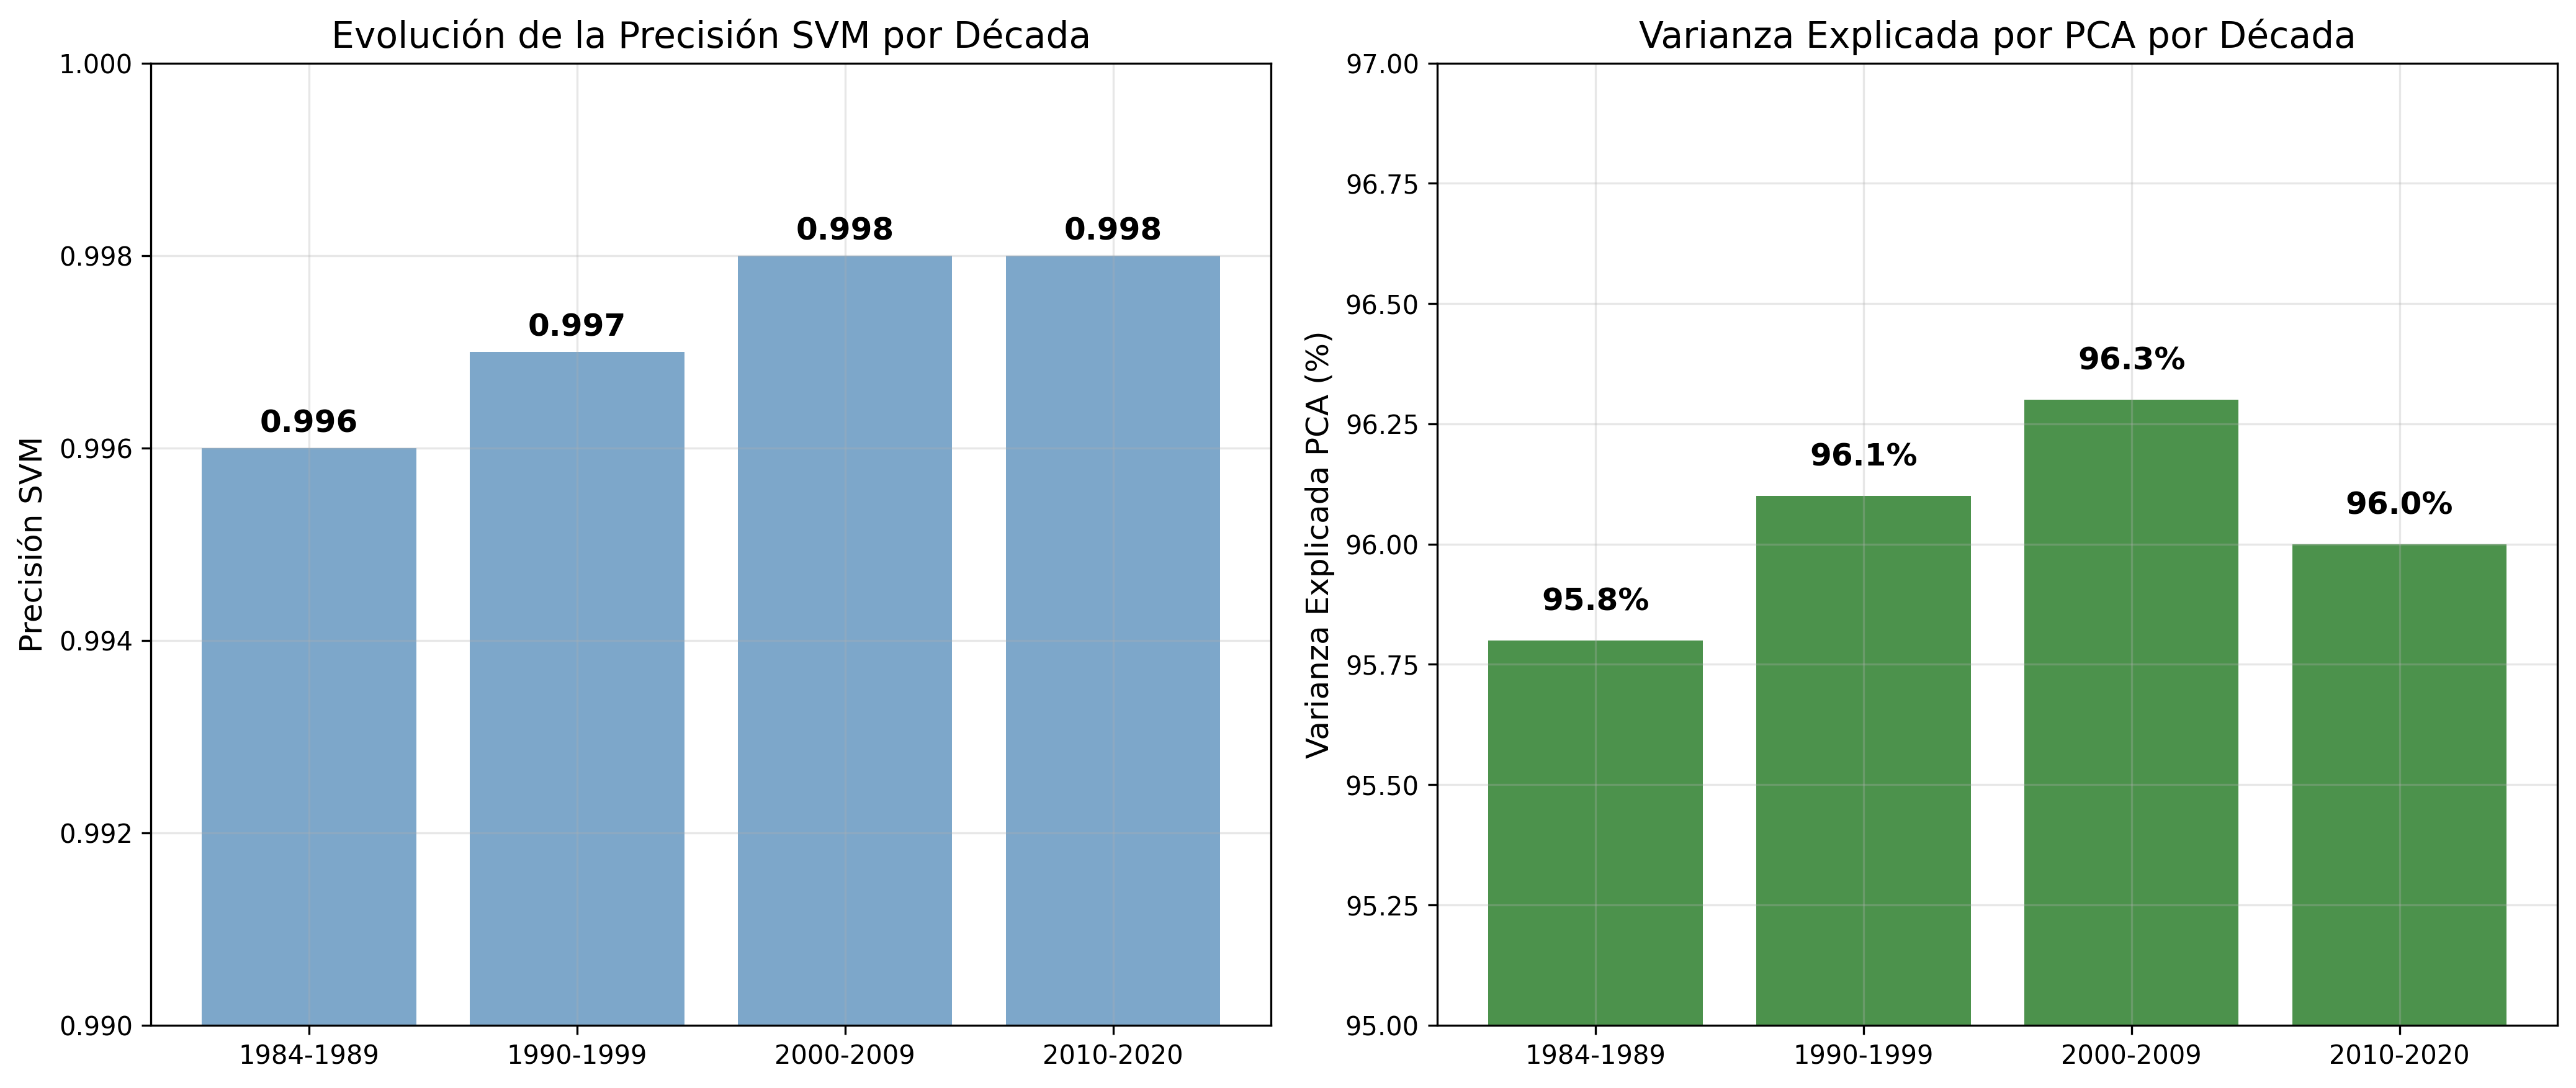
\includegraphics[width=\linewidth]{figures/temporal_quality_distribution.png}
\caption{Indicadores auxiliares de calidad por década, derivados del preprocesamiento de las capturas. No equivalen a control de calidad radiométrico de productos satelitales oficiales; sirven como apoyo visual para revisar la continuidad de la serie.}
\label{fig:quality_temporal}
\end{figure}

\subsection{Procedimiento de adquisición (Google Earth, imagen histórica)}

Las capturas se realizaron de forma \textbf{manual}: no hubo descarga masiva programática ni filtrado automático por metadatos de nubes en un servidor. El operador fijó la misma región de interés y, para cada año, avanzó en la \textbf{línea de tiempo histórica} hasta una fecha en la que la escena presentara poca nubosidad visible y buen contraste (meta equivalente al criterio de $<10\%$ de nubes indicado en la Tabla~\ref{tab:acquisition_stats}, pero aplicada por inspección visual). Posteriormente se exportó o capturó la imagen conservando el mismo encuadre entre años.

\begin{algorithm}
\caption{Procedimiento de adquisición manual con Google Earth}
\begin{algorithmic}[1]
\State Centrar el visor en la Zona Metropolitana de Querétaro y ajustar zoom, orientación y ángulo que se mantendrán fijos para toda la serie
\State Para cada año $y$ de 1984 a 2020:
	\State \quad Abrir la herramienta de \textit{imagen histórica} y seleccionar el año $y$
	\State \quad Desplazarse dentro del año hasta una fecha con cobertura nubosa baja (criterio visual)
	\State \quad Verificar que el encuadre coincide con el resto de la serie (sin desplazamientos accidentales)
	\State \quad Exportar o capturar la imagen y guardarla con nomenclatura estandarizada (p.\ ej.\ \texttt{YYYY.png})
\State Revisar visualmente la continuidad de la serie (saltos bruscos, años atípicos) y repetir la captura solo cuando una escena resulte claramente inutilizable
\end{algorithmic}
\end{algorithm}

\subsection{Control de calidad y representatividad}

En la adquisición, el control de calidad fue principalmente \textbf{visual} (nubosidad, sombras, nitidez, consistencia del encuadre). Ya conformada la carpeta de imágenes, el \textbf{pipeline de preprocesamiento} aplica comprobaciones reproducibles ---dimensiones homogéneas, formato RGB, detección de archivos faltantes y reescalado cuando una captura varió en resolución de pantalla--- antes de alimentar al clasificador; a ello se suman una validación geométrica (dimensiones consistentes y ajuste a la cuadrícula de referencia), una de intensidades (histogramas RGB para detectar anomalías evidentes, sin calibración radiométrica entre sensores) y una temporal (continuidad de la serie y sustitución puntual de años claramente anómalos). El conjunto final queda resumido en la Tabla~\ref{tab:acquisition_stats} y en la Figura~\ref{fig:quality_temporal}; se revisó de forma cualitativa que la serie cubra el perímetro metropolitano, años representativos del crecimiento documentado y una resolución temporal anual suficiente para el modelo celular. Esta revisión no equivale a una auditoría de sensores ni de catálogos de escenas, ya que las capturas provienen del visor de Google Earth.

\subsection{Limitaciones y mitigación}

El dataset tiene cuatro limitaciones principales: la resolución y nitidez efectivas dependen del nivel de zoom, del fondo cartográfico de cada fecha y de la compresión al exportar; el operador no controla la corrección atmosférica ni el origen exacto de cada tesela subyacente; la comparabilidad cromática entre años puede variar cuando el proveedor actualiza mosaicos; y el criterio de temporada seca y baja nubosidad es visual, no un filtrado por metadatos de nubes. Para acotar su impacto se fijaron los parámetros de vista (zoom, orientación, región) lo más constantes posible entre años, se homogeneizaron formato y dimensiones en el preprocesamiento, se hizo una revisión cruzada año con año para detectar saltos de contraste o nubosidad residual, y se normalizaron los valores de píxel con vistas a la clasificación binaria, sin pretender una calibración radiométrica entre sensores.

La Tabla~\ref{tab:uncertainty} organiza estas fuentes de error por tipo, con una estimación cualitativa de su nivel y de su efecto sobre los mapas binarios. Los niveles (bajo, medio, alto) son juicios del autor a partir de la inspección de la serie y no mediciones formales de incertidumbre; sirven para dar prioridad a las estrategias de mitigación y para acotar honestamente el alcance de los resultados.

\begin{table}[h]
\centering
\caption{Estimación cualitativa de las principales fuentes de error del conjunto de imágenes, su efecto sobre los mapas binarios y su mitigación. Los niveles son apreciaciones del autor, no medidas formales de incertidumbre.}
\begin{tabularx}{\textwidth}{|>{\raggedright\arraybackslash}p{0.18\textwidth}|>{\centering\arraybackslash}p{0.08\textwidth}|>{\raggedright\arraybackslash}X|>{\raggedright\arraybackslash}p{0.26\textwidth}|}
\hline
	\textbf{Tipo de error} & \textbf{Nivel} & \textbf{Efecto sobre los mapas} & \textbf{Mitigación aplicada} \\
\hline
Georreferenciación / encuadre & Bajo--medio & Pequeños desplazamientos entre capturas por reposicionamiento manual del visor; desalineación píxel a píxel entre años. & Mismo zoom, orientación y región; ajuste a la cuadrícula de referencia en el preprocesamiento. \\
\hline
Temporal (fecha intra-anual) & Medio & La fecha exacta varía dentro de cada año; cambios fenológicos y estacionales alteran la respuesta de la vegetación. & Captura preferente en temporada seca (nov.--abr.) y revisión de continuidad de la serie. \\
\hline
Mosaico / composición del proveedor & Medio--alto & Google Earth actualiza mosaicos y mezcla fuentes y fechas; discontinuidades de textura y color no atribuibles a cambio real. & Revisión cruzada año con año y sustitución puntual de escenas claramente anómalas. \\
\hline
Cromático / radiométrico & Medio & Sin corrección atmosférica; diferencias de balance de color e iluminación que sesgan los índices de color (NGRDI). & Normalización y estandarización por imagen; descriptores de textura (LBP) robustos a la iluminación. \\
\hline
Clasificación (LBP+K-Means+SVM) & Medio & Pseudoetiquetas no supervisadas, sin verdad terreno; ruido binario y sobre o subestimación local de lo urbano. & Validación interna \textit{train/test} y evaluación temporal indirecta del modelo AC (Capítulo~\ref{ch:resultados-analisis}). \\
\hline
\end{tabularx}
\label{tab:uncertainty}
\end{table}

\section{Pipeline de clasificación: de RGB a mapas binarios}

El preprocesamiento homogeneiza formato y dimensiones de las capturas RGB y prepara la entrada al clasificador automático (LBP+K-Means+SVM). El \textit{pipeline}, implementado en Python, encadena las etapas que resume la Figura~\ref{fig:preprocessing}:

Antes de describirlo conviene justificar por qué se eligió esta cadena y no un enfoque supervisado directo. La razón de fondo es que no se dispone de una verdad terreno etiquetada para los 37 años de la serie: un clasificador supervisado clásico o un \textit{Random Forest} exigiría etiquetar manualmente muestras representativas año por año, y una arquitectura profunda tipo U-Net necesitaría además grandes volúmenes anotados y cómputo en GPU, sin aportar interpretabilidad sobre la decisión urbano/no-urbano. Frente a ello, la cadena combina texturas y color de forma no supervisada: los patrones binarios locales (LBP) describen la rugosidad del tejido construido y son robustos a cambios de iluminación, el agrupamiento K-Means genera pseudoetiquetas sin información previa, y un SVM lineal consolida a partir de ellas una frontera de decisión reproducible y ligera. Dado que el problema es binario y que las imágenes son RGB sin banda infrarroja, este contraste de textura y color basta para separar lo construido de lo no construido; la opción elegida es, además, computacionalmente liviana (sin GPU) y replicable, lo que prioriza la reproducibilidad sobre una exactitud marginalmente mayor que las alternativas más pesadas no garantizan en ausencia de etiquetas.

\begin{figure}[H]
\centering
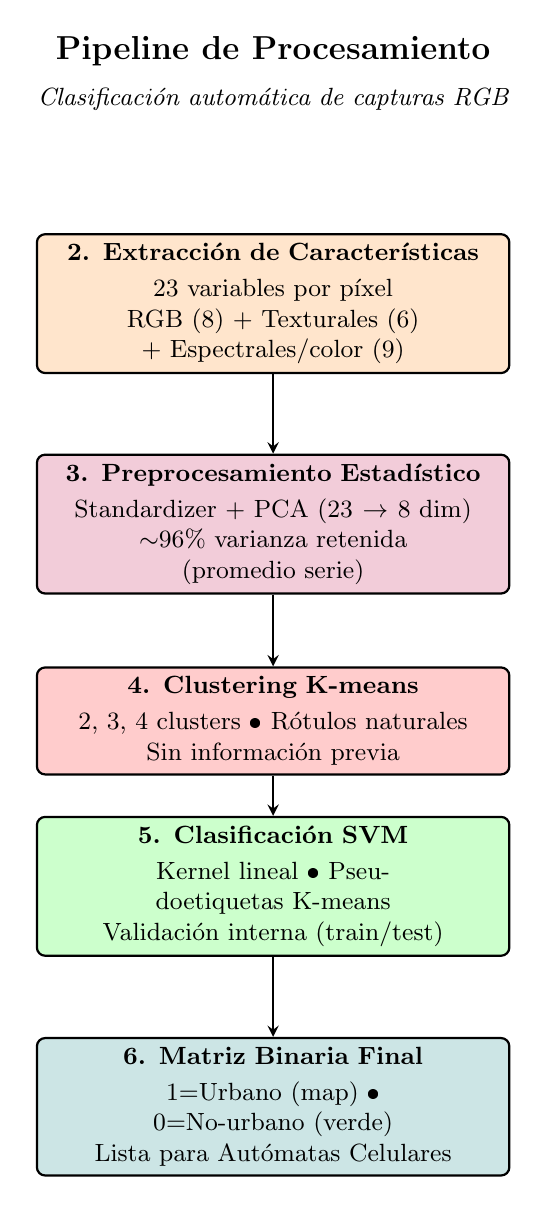
\begin{tikzpicture}[
	node distance=1.2cm,
	box/.style={
		rectangle,
		rounded corners=3pt,
		draw=black,
		thick,
		minimum width=6cm,
		minimum height=1cm,
		text width=5.5cm,
		align=center,
		font=\small
	},
	step1/.style={box, fill=blue!20},
	step2/.style={box, fill=orange!20},
	step3/.style={box, fill=purple!20},
	step4/.style={box, fill=red!20},
	step5/.style={box, fill=green!20},
	step6/.style={box, fill=teal!20},
	arrow/.style={-stealth, thick},
	label/.style={circle, fill=white, draw=black, thick, font=\bfseries, minimum size=0.8cm}
]

% Título del pipeline
\node[font=\bfseries\large] at (0, 0) {Pipeline de Procesamiento};
\node[font=\small\itshape, text width=6cm, align=center] at (0, -0.6) {Clasificación automática de capturas RGB};

% Paso 2: Extracción de Características
\node[step2] (step2) at (0, -3.2) {
	\textbf{2. Extracción de Características}\\[2pt]
	23 variables por píxel\\
	RGB (8) + Texturales (6) + Espectrales/color (9)
};


% Paso 3: Preprocesamiento Estadístico
\node[step3] (step3) at (0, -6.0) {
	\textbf{3. Preprocesamiento Estadístico}\\[2pt]
	Standardizer + PCA ($23\to 8$ dim)\\
	$\sim$96\% varianza retenida (promedio serie)
};


% Paso 4: Clustering K-means
\node[step4] (step4) at (0, -8.5) {
	\textbf{4. Clustering K-means}\\[2pt]
	2, 3, 4 clusters • Rótulos naturales\\
	Sin información previa
};


% Paso 5: Clasificación SVM
\node[step5] (step5) at (0, -10.6) {
	\textbf{5. Clasificación SVM}\\[2pt]
	Kernel lineal • Pseudoetiquetas K-means\\
	Validación interna (train/test)
};


% Paso 6: Matriz Binaria Final
\node[step6] (step6) at (0, -13.4) {
	\textbf{6. Matriz Binaria Final}\\[2pt]
	1=Urbano (map) • 0=No-urbano (verde)\\
	Lista para Autómatas Celulares
};


% Flechas de conexión
\draw[arrow] (step2) -- (step3);
\draw[arrow] (step3) -- (step4);
\draw[arrow] (step4) -- (step5);
\draw[arrow] (step5) -- (step6);

\end{tikzpicture}
\caption{Pipeline de preprocesamiento implementado}
\label{fig:preprocessing}
\end{figure}

\subsection{Extracción de características}

Para cada píxel, el código extrae automáticamente 23 características (implementación en \texttt{tesis\_ac.pipeline.feature\_extraction}, clase \texttt{FeatureExtractor}), organizadas en tres categorías:

\begin{table}[h]
\centering
\caption{Características extraídas por píxel a partir de cada captura RGB.}
\begin{tabular}{|l|c|p{8cm}|}
\hline
	\textbf{Categoría} & \textbf{Cantidad} & \textbf{Características específicas} \\
\hline
Básicas & 8 & Canales R, G, B; intensidad; brillo; desviación estándar de R, G y B. \\
\hline
Texturales & 6 & Sobel horizontal y vertical; magnitud del gradiente; LBP uniforme ($R = 3$, $P = 24$) sobre escala de grises; entropía local; contraste local. \\
\hline
Espectrales / color & 9 & Índice verde--rojo normalizado $(G-R)/(G+R)$; exceso de verde y exceso de rojo; componentes L, a, b (LAB); H, S, V (HSV). \\
\hline
	\textbf{Total} & \textbf{23} & \\
\hline
\end{tabular}
\label{tab:features}
\end{table}

Sobre la categoría espectral conviene una aclaración. Como las capturas son RGB y no incluyen banda infrarroja, aquí no se calcula un NDVI en sentido estricto: ese índice necesita el infrarrojo cercano, del que estas imágenes carecen. Lo que se usa son índices construidos únicamente con los canales visibles. El que se reporta como índice verde--rojo normalizado responde a la forma $(G-R)/(G+R)$ y coincide con el NGRDI que la literatura de percepción remota emplea con cámaras RGB; junto con el exceso de verde y de rojo cumple el papel de un proxy cromático de vegetación, suficiente para separar superficies vegetadas de las construidas a partir del contraste de color, que es lo que requiere la clasificación binaria de este trabajo.

\subsection{Normalización y reducción dimensional}

El preprocesamiento incluye dos etapas adicionales antes del clasificador:

\begin{enumerate}
	\item \textbf{Normalización estadística}: aplicación de \texttt{StandardScaler} para centrar y escalar cada característica.
	\item \textbf{Reducción dimensional}: análisis de componentes principales (PCA) para pasar de 23 a 8 componentes.
\end{enumerate}

La PCA retiene en promedio cerca del $96$\,\% de la varianza original, una compresión razonable sin pérdida apreciable de información para la clasificación binaria. La Tabla~\ref{tab:preprocessing_quality} resume el preprocesamiento aplicado a toda la serie.

\begin{table}[h]
\centering
\caption{Resumen agregado del preprocesamiento aplicado a la serie 1984--2020.}
\begin{tabularx}{\textwidth}{|>{\raggedright\arraybackslash}p{0.35\textwidth}|X|}
\hline
	\textbf{Métrica} & \textbf{Valor} \\
\hline
Varianza retenida por PCA (promedio de la serie) & Cerca del $96$\,\%. \\
Componentes finales por píxel & 8 (a partir de los 23 descriptores originales). \\
Características válidas por imagen & 23 de 23 (ningún descriptor se descarta). \\
Píxeles procesados por imagen & $5{,}419{,}008$ ($1{,}792 \times 3{,}024$). \\
\hline
\end{tabularx}
\label{tab:preprocessing_quality}
\end{table}

La implementación se organiza en una arquitectura modular ---rasterización/clasificación de las capturas, cálculo de Pesos de Evidencia y simulación con autómatas celulares--- cuyo diagrama de clases UML y rutas de los módulos del repositorio se documentan en el Apéndice~\ref{ap:arquitectura}, para no recargar la descripción metodológica.

En este espacio RGB enriquecido con descriptores de textura ---en particular los patrones binarios locales (LBP) de \textcite{Ojala2002}, robustos a cambios de iluminación y útiles para distinguir la rugosidad del tejido construido---, los primeros componentes del PCA reflejan el contraste urbano--vegetación y la variabilidad local, de modo que el SVM trabaja sobre representaciones comprimidas y poco redundantes.

% Fuente: report/tesis/book/cap03/analisis-datos.tex
\section{Análisis de datos procesados y transformación binaria}

Esta sección resume la salida del pipeline: mapas binarios anuales urbano/no-urbano listos para alimentar el modelo WoE--AC del capítulo siguiente.

\subsection{Resultados de la transformación binaria}

La \figref{fig:binary_evolution} muestra la evolución temporal del crecimiento urbano de Querétaro capturada mediante la clasificación binaria.

\begin{figure}[ht]
	\centering
	\begin{subfigure}[b]{0.32\textwidth}
			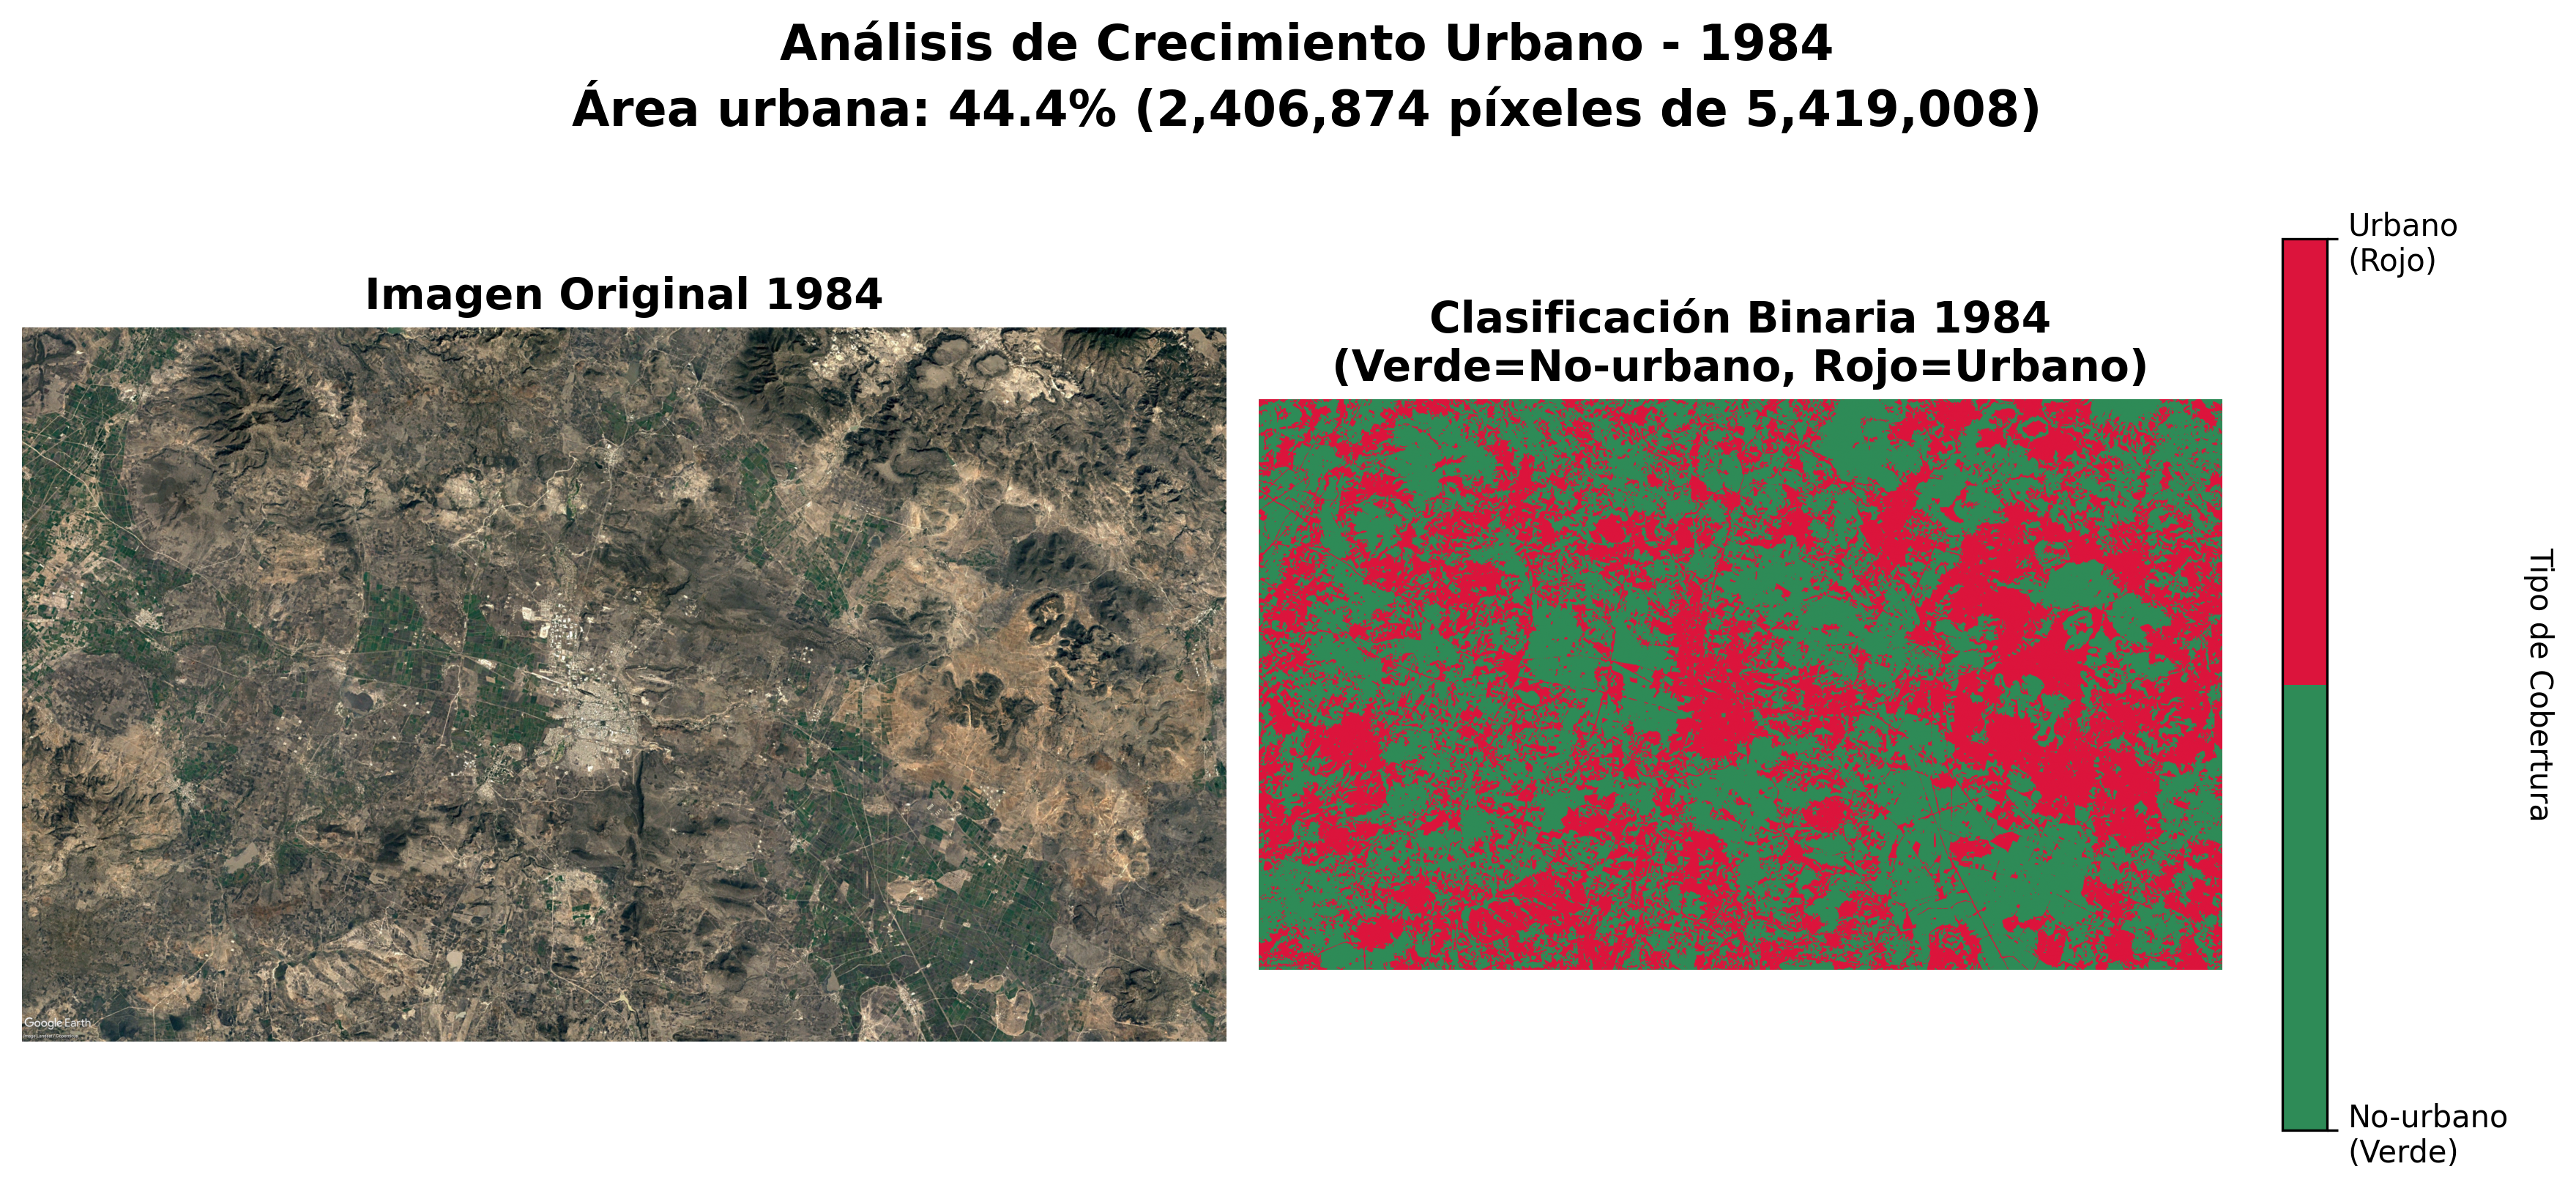
\includegraphics[width=\textwidth]{figures/binary_transformation_1984.png}
		\caption{1984 - Estado inicial}
		\label{fig:binary_1984}
	\end{subfigure}
	\hfill
	\begin{subfigure}[b]{0.32\textwidth}
			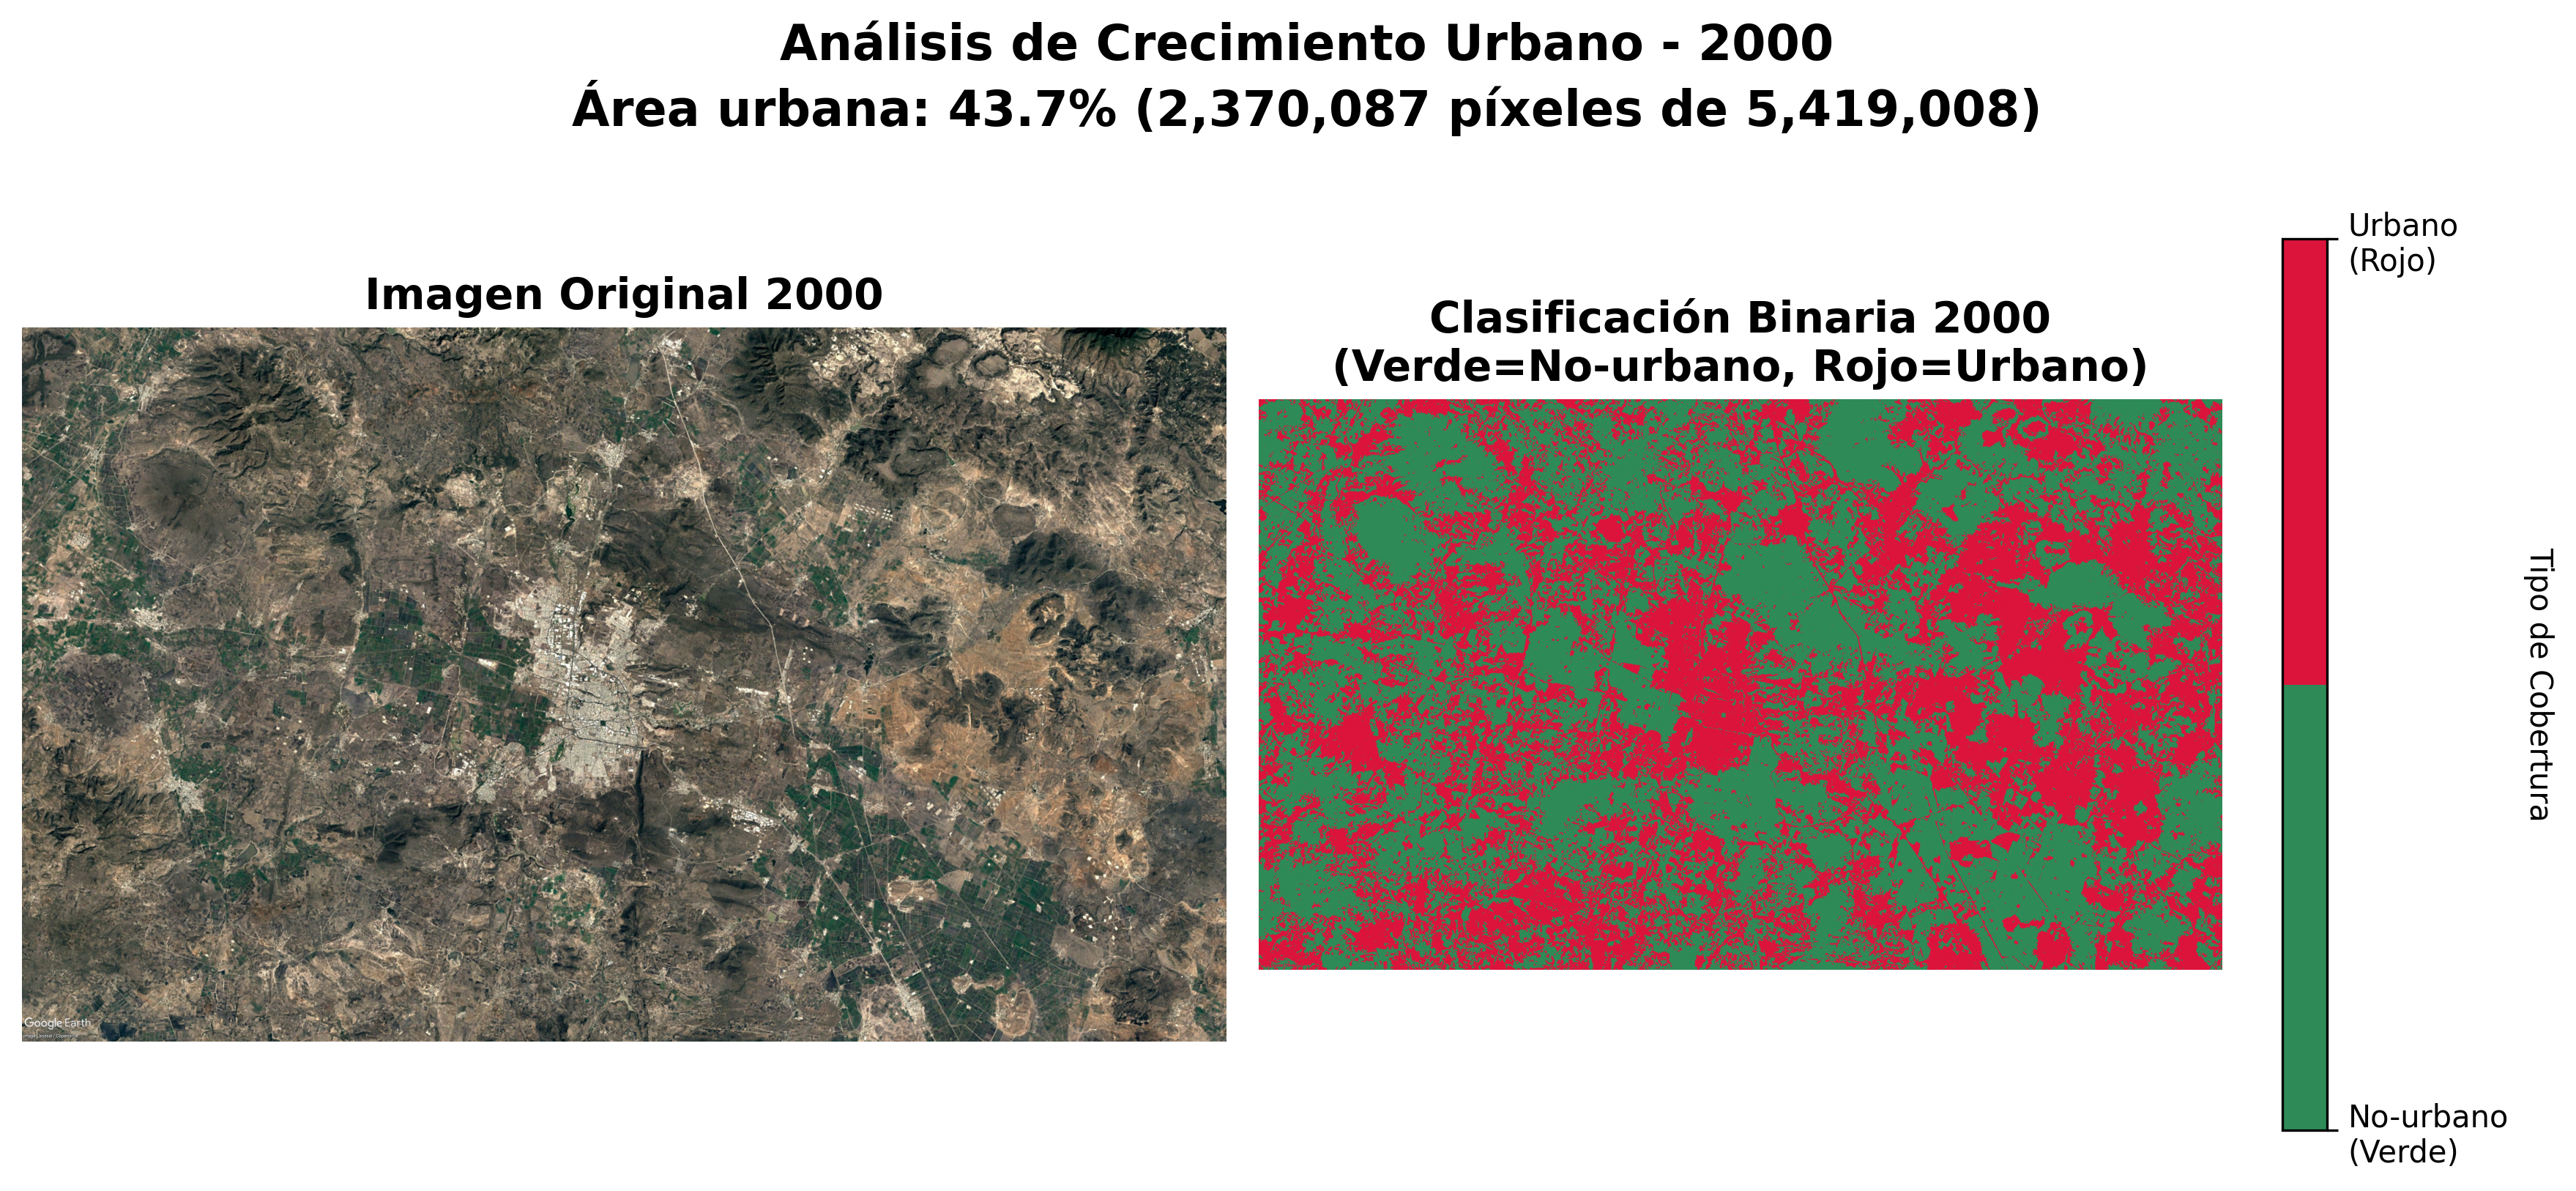
\includegraphics[width=\textwidth]{figures/binary_transformation_2000.png}
		\caption{2000 - Expansión intermedia}
		\label{fig:binary_2000}
	\end{subfigure}
	\hfill
	\begin{subfigure}[b]{0.32\textwidth}
			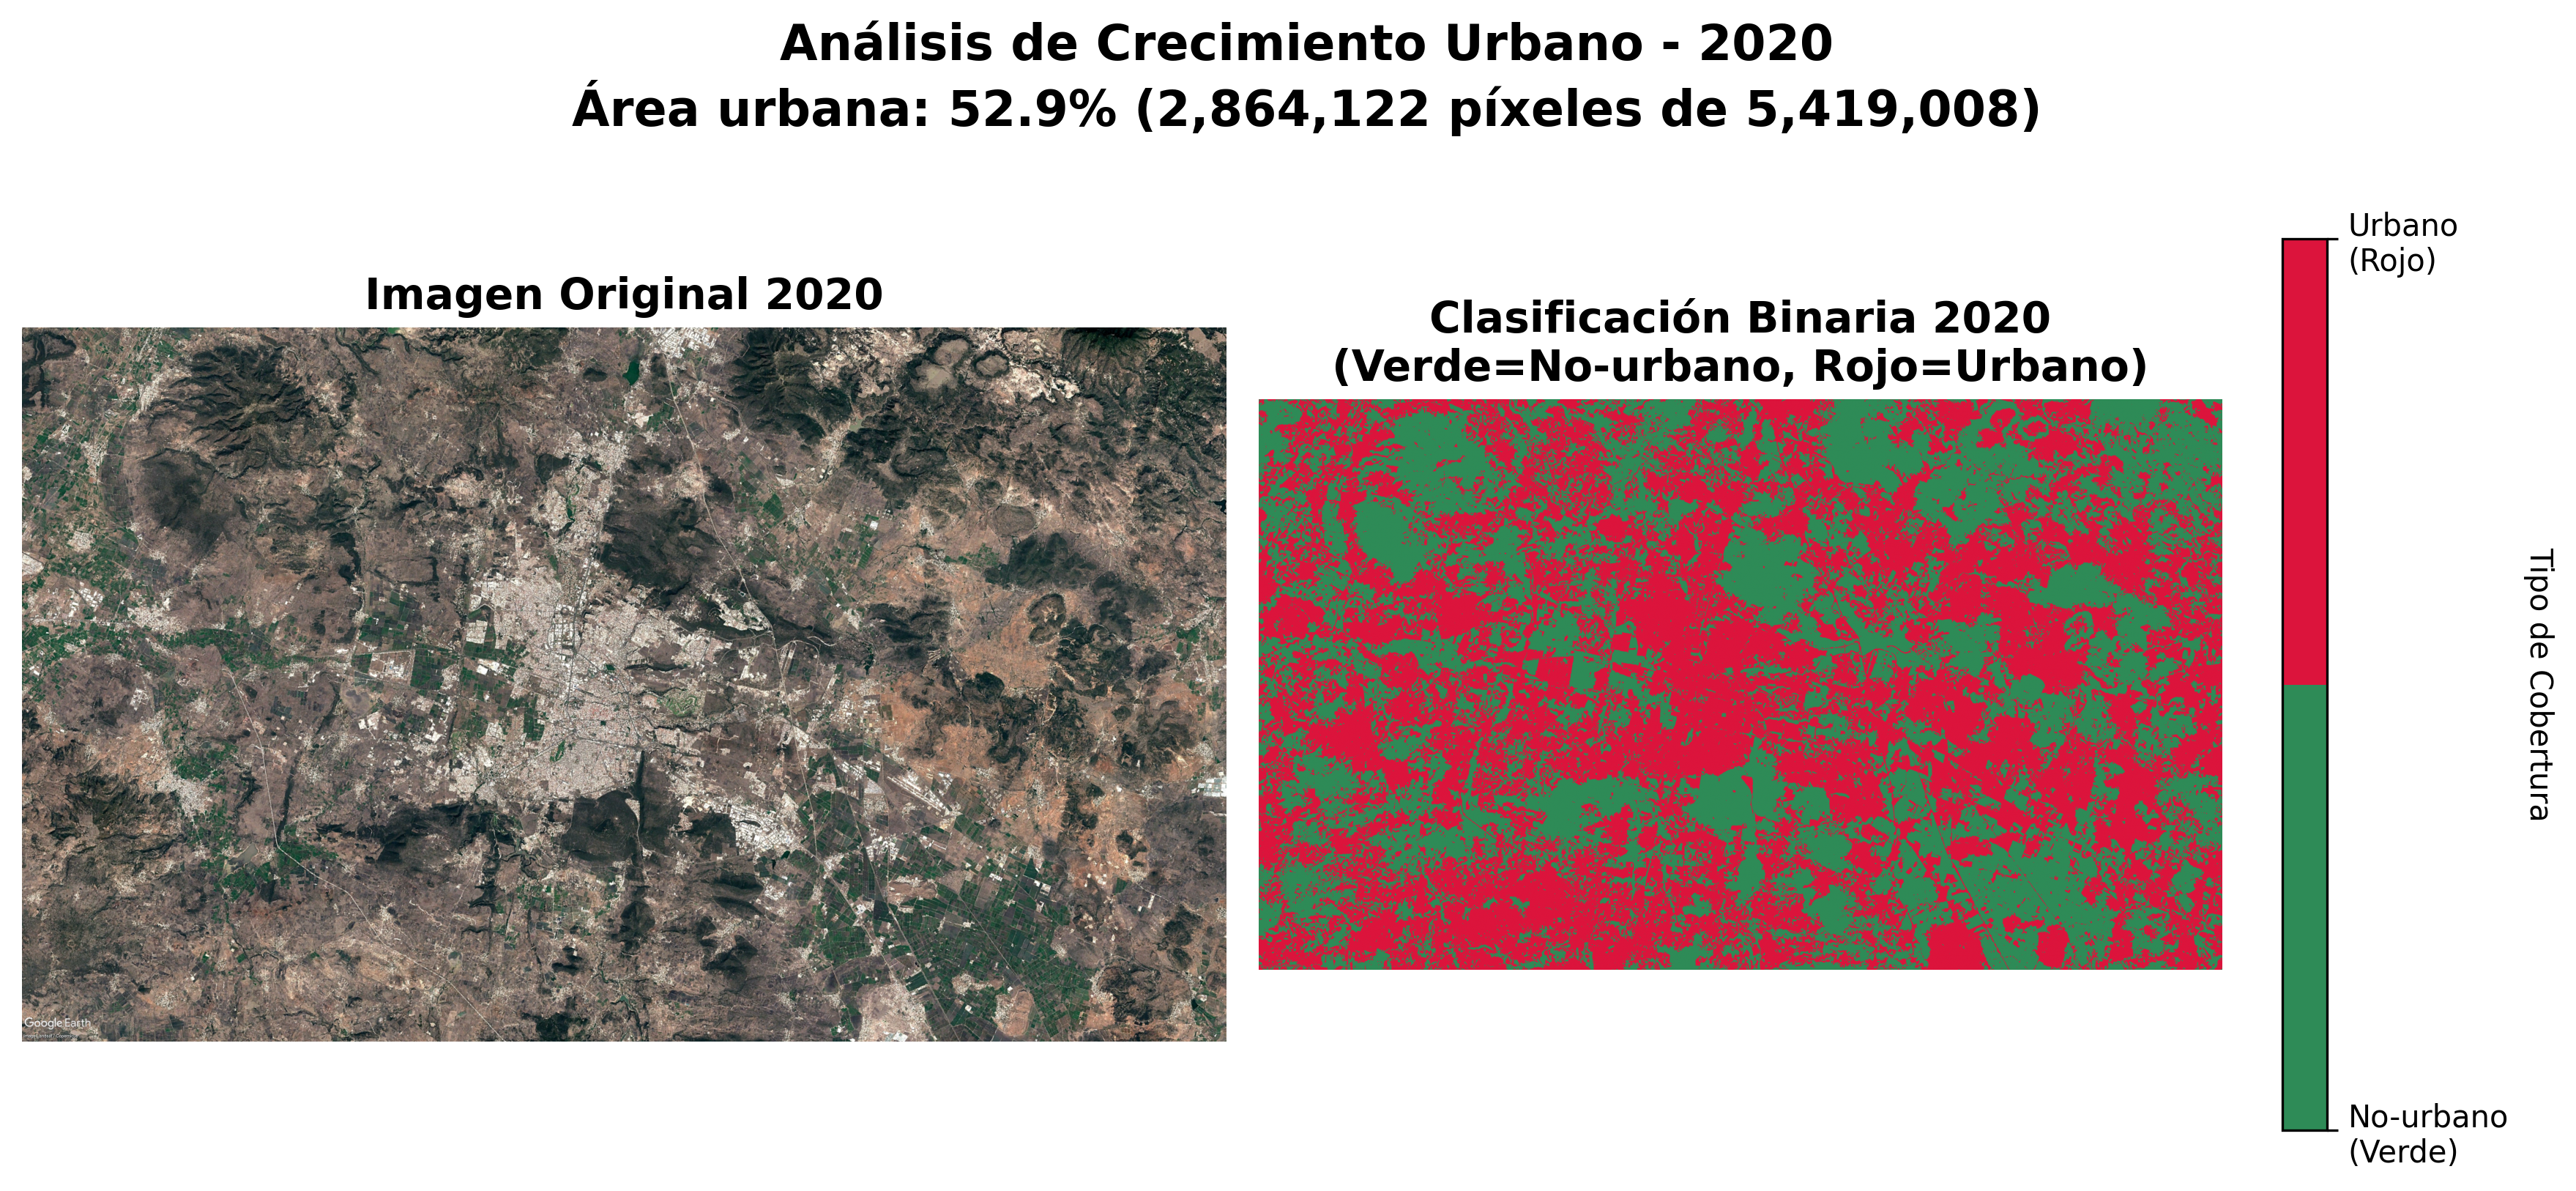
\includegraphics[width=\textwidth]{figures/binary_transformation_2020.png}
		\caption{2020 - Estado actual}
		\label{fig:binary_2020}
	\end{subfigure}
	\caption{Evolución del crecimiento urbano de la Zona Metropolitana de Querétaro (1984--2020), representada mediante mapas binarios urbano/no-urbano obtenidos a partir de la clasificación LBP+K-Means+SVM aplicada a las capturas RGB de la serie.}
	\label{fig:binary_evolution}
\end{figure}

\subsection{Calidad interna de la clasificación}

La calidad del clasificador LBP+K-Means+SVM se evalúa con un reparto interno \textit{train/test} ($20$\,\% para prueba por defecto) sobre las pseudoetiquetas generadas por K-Means, conforme a la rutina de entrenamiento de \texttt{ImageClassifier} en el repositorio. En los experimentos sobre Querétaro, la concordancia del SVM con esas pseudoetiquetas ---medida como \textit{accuracy} en el reparto interno, no contra una verdad terreno--- se situó en el rango $88$--$94$\,\%, en línea con lo comentado en el Capítulo~\ref{ch:modelo-crecimiento-urbano}.

Este porcentaje mide la coherencia interna del clasificador ---es decir, qué tan bien el SVM reproduce las etiquetas generadas por K-Means--- y no la exactitud respecto a una verdad terreno externa independiente. La validación externa del \textit{pipeline} se realiza, de manera indirecta, a través de la evaluación temporal del modelo AC en el Capítulo~\ref{ch:resultados-analisis}.

\subsection{Justificación de la representación binaria}

La simplificación del mapa de cobertura de suelo a dos categorías (urbano/no-urbano) responde a tres consideraciones metodológicas:

\begin{enumerate}
	\item \textbf{Compatibilidad con el AC}: Los Autómatas Celulares utilizados en este trabajo operan con estados discretos. La representación binaria elimina la necesidad de una etapa adicional de discretización y hace que las reglas de transición sean directamente interpretables.

	\item \textbf{Disponibilidad de datos}: Las capturas disponibles son RGB; no se incorporan bandas térmicas ni radar. Esa restricción acota la discriminación fina de usos intraurbanos y hace razonable condensar la salida en dos clases.

	\item \textbf{Objetivo del modelo}: El interés del trabajo es modelar la \textit{expansión} del área urbana, no la composición interna de usos de suelo. La clasificación binaria captura la variable de salida relevante para este propósito.
\end{enumerate}

\subsection{Síntesis del capítulo}

La inspección visual de los mapas binarios anuales (Figura~\ref{fig:binary_evolution}) muestra transiciones graduales y continuas entre años consecutivos, con patrones de expansión congruentes con el crecimiento documentado para la ZMQ, sin artefactos sistemáticos ni discontinuidades espaciales abruptas en la serie.

Este capítulo describió la zona de estudio, la obtención manual de imágenes con Google Earth (línea de tiempo histórica) y el pipeline de clasificación LBP+K-Means+SVM que transforma las imágenes RGB en mapas binarios anuales. La serie resultante de 37 mapas (1984--2020) constituye la entrada principal para el cálculo de los Pesos de Evidencia y la simulación con Autómatas Celulares descritos en el capítulo siguiente.
